\section{Implementierung eines naiven Bayes-Klassifikators}
    Basierend auf den theoretischen Grundlagen aus Kapitel~\ref{sec:theory} sollen nun in diesem Kapitel die Implementierung eines naiven Bayes-Klassifikators zur Textklassifikation sowie einige zu beachtende Besonderheiten behandelt werden.

    \subsection{Projektbeschreibung}
        Um die bisher behandelten theoretischen Grundlagen umzusetzen und zu testen wurde in der Klasse \textit{NaiveBayesClassificator} ein naiver Bayes-Klassifikator implementiert.

        Dieser verwendet ein Unigram-Wortsequenz-Modell, um Daten aus verschiedenen Kategorien in \textit{nltk.corpus.brown.tagged\_sents} zu klassifizieren.

        Dazu wird der \textit{train}-Methode des Klassifikators eine Liste von Dokumenten verschiedener Themen, sowie eine Liste mit zugehörigen Klassenlabels übergeben, mit deren Hilfe der Klassifikator eine Entscheidungsfunktion $\gamma$~lernt.

        Ein Aufruf der \textit{predict}-Methode mit einem Dokument als Argument klassifiziert dieses anhand der erlernten Entscheidungsfunktion.

        Mittels der \textit{info}-Methode des Klassifikators hat man die Möglichkeit, eine Liste der $n$ wichtigsten Wörter einer Dokumentenklasse ausgeben zu lassen.
        \newline
        
        Zur Bestimmung der Genauigkeit des Klassifikators wurde in der Klasse \textit{Evaluator} die Möglichkeit einer k-fachen Kreuzvalidierung implementiert.
        Dabei werden die übergebenen Daten in $k$ Segmente eingeteilt, wovon $k-1$ Segmente zum Training und ein Segment zum Test des Klassifikators verwendet werden.
        Bildet man anschließend den Mittelwert über $k$ Genauigkeitswerten, lassen sich auch bei kleinen Datensätzen aussagekräftige Werte über die Genauigkeit des Klassifikators ermitteln.

    \subsection{Textklassifikationspipeline}
        Grundsätzlich kann der Vorgang der Textklassifikation, wie in Abbildung~\ref{fig:pipeline} dargestellt, in vier Schritte eingeteilt werden.

        \begin{figure}[htpb]
            \centering
            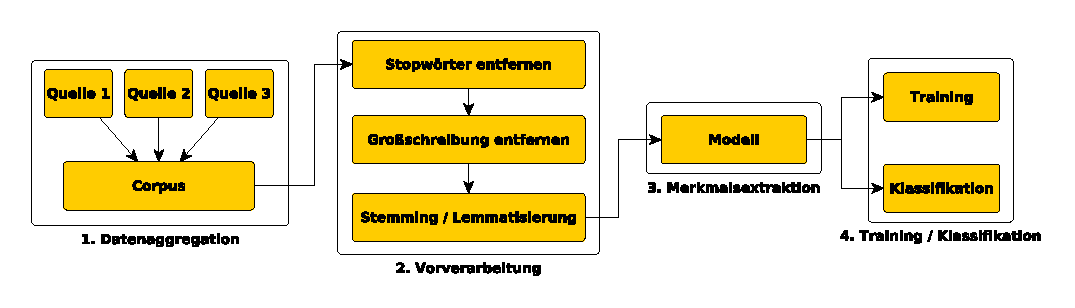
\includegraphics[scale=.80]{images/classification_pipeline_horizontal}
            \caption{Einzelschritte der Textklassifikation}\label{fig:pipeline}
        \end{figure}

        Der folgende Abschnitt beschreibt, wie die einzelnen Teilschritte der Pipeline im Rahmen dieser Seminararbeit implementiert wurden.

        \subsubsection{Datenaggregation}
            Zum Trainieren und Testen des Klassifikators werden Daten aus dem NLTK Brown Corpus verwendet. Darin enthalten sind Sätze verschiedener Themengebiete, welche als Liste einzelner Wörter vorliegen. 

            Die Implementierung des Klassifikators akzeptiert Daten in diesem Format, somit müssen keine weiteren Verarbeitungsschritte zur Datenaufbereitung vorgenommen werden.

        \subsubsection{Vorverarbeitung}
            Bevor Merkmale aus den Daten extrahiert werden, durchlaufen sie einen Vorverarbeitungsschritt, der die Eingangsdaten filtert und aufbereitet. 
            Dies geschieht in der vorliegenden Implementierung mit Hilfe der Klasse \textit{Preprocessor}, welche folgende Aufgaben übernimmt:\newline\newline
            \textbf{Stopwörter entfernen}:\newline
            Elemente natürlicher Sprache lassen sich bezüglich ihres Informationsgehalts unterscheiden. 
            Viele so genannte ``Füllwörter'' treten häufig auf, liefern allerdings keinen Mehrwert an Information bezüglich der Bedeutung eines Satzes bzw. Textes. 
            Da diese Füllwörter den Merkmalsraum eines Dokuments unnötig vergrößern, werden sie im Allgemeinen vor der Klassifikation entfernt~\cite{nltk}. 
            Die NLTK-Bibliothek beinhaltet zu diesem Zweck Wörterbücher mit Füllwörtern verschiedener Sprachen, welche in der Methode \textit{remove\_stopwords} verwendet werden, um diese aus den Daten zu entfernen.\newline\newline
            \textbf{Lemmatisierung}:\newline
            Durch Lemmatisierung wird versucht, die unterschiedlich gebeugten Formen eines Wortes in einem Dokument auf ihr Lemma zurückzuführen, um eine unnötige Vergrößerung des Merkmalsraumes zu vermeiden~\cite{IIR}.

            Dies wird mit Hilfe des in NLTK enthaltenen \textit{WordNetLemmatizer} erreicht, welcher sich in \textit{nltk.stem.wordnet} befindet und auf Daten von WordNet zurückgreift.\newline\newline
            \textbf{Interpunktion entfernen}:\newline
            Die in NLTK enthalten Daten beinhalten neben einzelnen Wörtern auch vollständige Interpunktion. 

            Da die unabhängig von der Dokumentenklasse häufig auftretenden Satzzeichen die Liste der für eine Klasse signifikanten Merkmale verfälschen würden, werden Merkmale, die in \textit{string.punctuation} enthalten sind, entfernt.\newline\newline
            \textbf{Großschreibung entfernen}:\newline
            Die Datensätze in \textit{nltk.corpus.brown.tagged\_sents} liegen in korrekter Groß- und Kleinschreibung vor. 
            Da für die Klassifikation nach Themengebiet die Groß- und Kleinschreibung keine signifikante Rolle spielt, werden die Eingangsdaten im Prozess der Vorverarbeitung auf Kleinschreibung vereinheitlicht.

        \subsubsection{Merkmalsextraktion}
                Nachdem die Eingangsdaten erfolgreich vorverarbeitet wurden, können im Schritt der Merkmalsextraktion klassifizierbare Merkmale daraus extrahiert werden. 
                Dabei wird mittels eines Sets ein Vokabular der Trainingsdaten erstellt (siehe Abschnitt~\ref{sec:vocab}), welches zur Erstellung der Merkmalsvektoren verwendet wird.

        \subsubsection{Training / Klassifikation}
                Im letzten Schritt der Pipeline wird nun entweder ein neuer Klassifikator anhand der aus Dokumenten extrahierten Merkmale trainiert, oder eben diese Dokumente werden mittels eines bereits trainierten Klassifikators klassifiziert. 
                
                Das prinzipielle Vorgehen dabei ist in Abbildung~\ref{fig:algo} dargestellt.

        \begin{figure}[htpb]
            \centering
            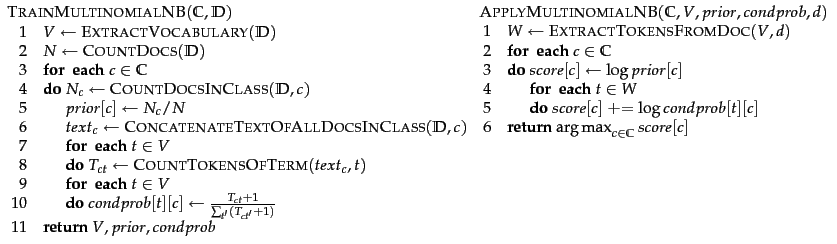
\includegraphics[scale=0.5]{images/algo2.png}
            \caption{Algorithmen für Training und Klassifikation\newline\tiny{Quelle: http://nlp.stanford.edu/IR-book/html/htmledition/naive-bayes-text-classification-1.html}}\label{fig:algo}
        \end{figure}

    \subsection{Arithmetischer Unterlauf}\label{sec:log}
    Anhand von Gleichung~\ref{eq:cond_prod} lässt sich erkennen, dass die bedingte Wahrscheinlichkeit $\hat{P}(\mathbf{x}|c)$ ein Produkt mehrerer Wahrscheinlichkeiten mit Werten im Bereich $0 \le x \le 1$ ist.

    Aufgrund der endlichen Genauigkeit der Gleitkommadarstellung von Computern kann es hierbei allerdings zu einem arithmetischen Unterlauf kommen und $\hat{P}(\mathbf{x}|c)$ wird zu $0$ gerundet. Um dieses Problem zu umgehen, bietet es sich an, mit logarithmierten Wahrscheinlichkeiten zu arbeiten~\cite{IIR}.
        
        Dadurch ergibt sich Gleichung~\ref{eq:class_bayes_3} zu:

        \begin{equation}
            c_{m} = \argmax_{c \in K}\left[\log{\hat{P}(c)} + \sum_{i=1}^{n}\log{\hat{P}(x_{i}|c)}\right]
            \label{eq:log_bayes}
        \end{equation}

    \subsection{Additive Smoothing}
    Eine ähnliche Problemstellung zu Abschnitt~\ref{sec:log} ergibt sich, wenn im Trainingsdatensatz ein Merkmal enthalten ist, das explizit nur in einer Dokumentenklasse~$c_{k}$ auftritt. Dieses Merkmal hätte somit in allen anderen Dokumentenklassen eine Wahrscheinlichkeit $\hat{P}(x_{i}|c = \neg c_{k}) = 0$.

        Dies hätte zur Folge, dass, ausgehend von Gleichung~\ref{eq:class_bayes_3}, das Produkt~\ref{eq:cond_prod} nur für Dokumentenklasse~$c_{k}$ ein Ergebnis ungleich~$0$ liefern würde und somit~$c_{k}$ stets als passendste Dokumentenklasse gewählt wird~\cite{IIR}.

        %Bei Verwendung von Gleichung~\ref{eq:log_bayes} hingegen würde der Ausdruck~$\log{(0)}$ ausgewertet werden, welcher nicht definiert ist.

        Um dieses Problem der ``Nullwahrscheinlichkeiten'' zu eliminieren, wird häufig sogenanntes ``additive smoothing'' angewandt.
        Dabei wird ein beliebiger Wert $\epsilon$ zur Anzahl des Vorkommens eines Merkmals addiert, um damit das Auftreten einer Nullwahrscheinlichkeit zu verhindern.

        Gleichung~\ref{eq:cond_prob_xi} ändert sich dadurch zu:

        \begin{equation}
            \hat{P}(x_{i}|c) = \frac{\left[\sum_{\mathbf{x} \in c}\sum_{x_{i} \in \mathbf{x}}1\right]+\epsilon}{\sum_{\mathbf{x} \in c}\left[\sum_{w \in \mathbf{x}}1+\epsilon\right]}
            \label{eq:add_one}
        \end{equation}

    \subsection{Evaluation}
        Um die Genauigkeit des implementierten Klassifikators zu ermitteln, wird mit Hilfe der Klasse \textit{Evaluator} eine k-fache Kreuzvalidierung durchgeführt. 

        Die durchschnittliche Genauigkeit des Klassifikators, welche durch eine 5-fache Kreuzvalidierung mit Daten der Kategorien \textit{humor} und \textit{learned} ermittelt wurde, beträgt dabei 88\%.
